%
%  progress-presentation.tex
%  src
%
%  Created by Illya Starikov on 09/16/17.
%  Copyright 2017. Illya Starikov. All rights reserved.
%

% \documentclass[notes,xcolor=dvipsnames]{beamer}       % print frame + notes
% \documentclass[notes=only,xcolor=dvipsnames]{beamer}  % only notes
\documentclass[xclolor=dvipsnames]{beamer}            % only frames
%\documentclass[handout,xclolor=dvipsnames]{beamer}    % only frames, no pauses
\usepackage{soul,graphics}

\usepackage{amssymb,amsmath,verbatim,graphicx,microtype,upquote,units,booktabs,akkwidepage}

\newcommand{\chapterNumber}[1]{
    \setcounter{section}{#1}
    \addtocounter{section}{-1}
}
\title{Financial Planning (Presentation \#10)}
\subtitle{Special Topics (CS3001)}
\author{Illya Starikov}
\date{Sometimes In The Future}
\institute{Missouri University of Science and Technology}

\begin{document}
\begin{darkframes}
    \maketitle

    \begin{frame}
        \frametitle{A Brief Introduction}

        I have always had a problem with being financially responsible. As I am about to graduate, and will have exponentially more bills, I want a way to be able to handle all of them reasonably. So, I decided I needed a budget.
    \end{frame}

    \begin{frame}
        \frametitle{A Brief Introduction}

        I knew I would need a tool to help budget; after some search, I settled on EmPower. I also knew I needed something to invest money into, so I settled on Acorns.
    \end{frame}

    \begin{frame}
        \frametitle{A Brief Introduction}
        \subtitle{EmPower}

        \begin{figure}[H]
            \centering
            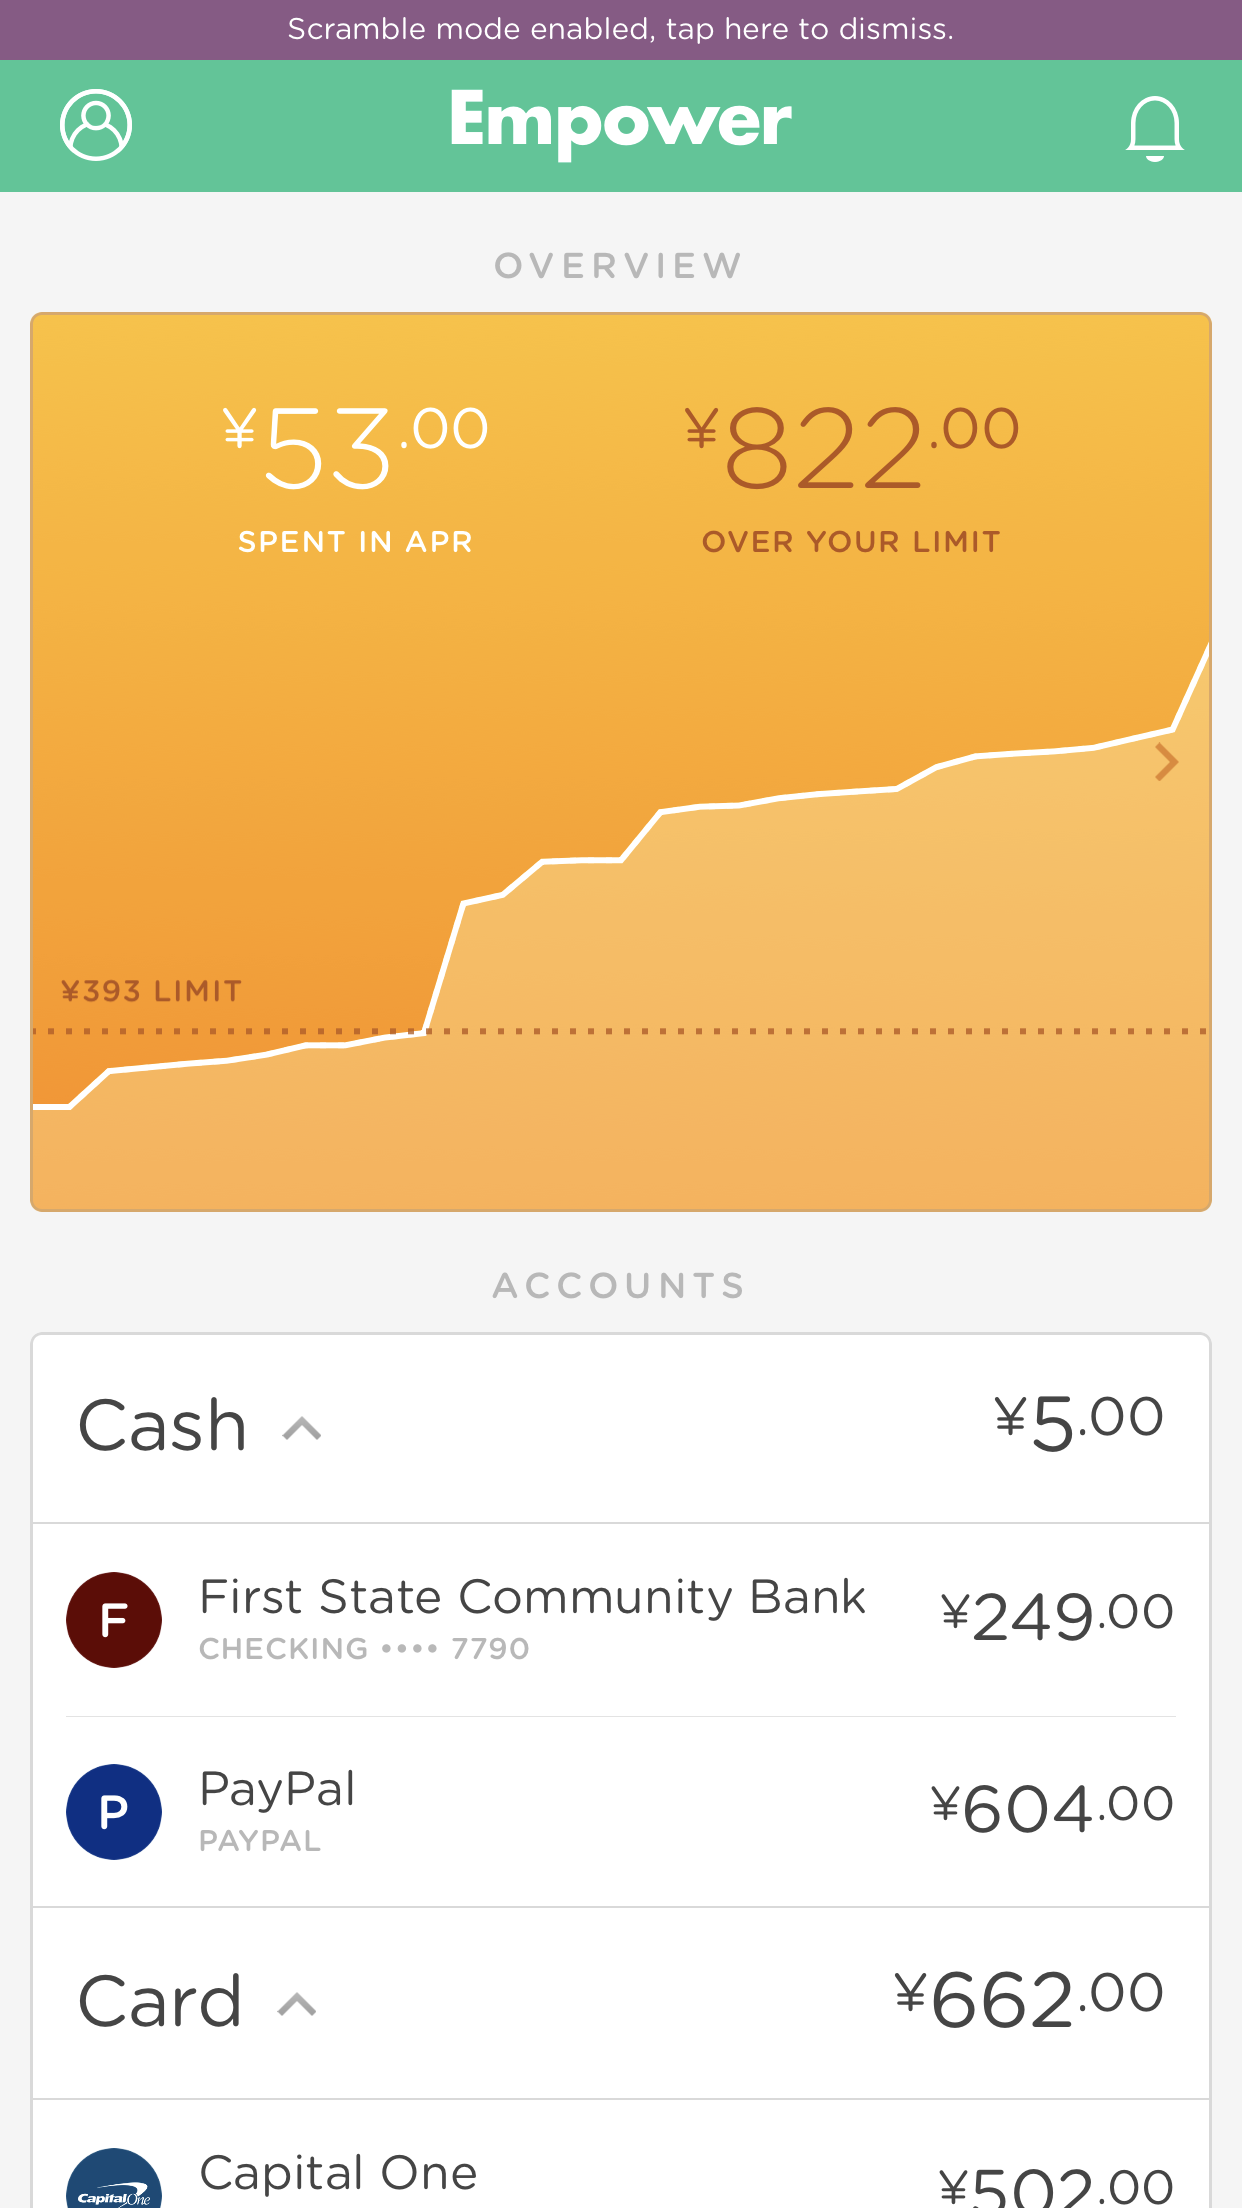
\includegraphics[height=.65\textheight]{assets/empower.png}
            \caption{Empower (With Scramble Mode On, So All Data Is Randomize)}
            \label{fig:empower}
        \end{figure}
    \end{frame}

    \begin{frame}
        \frametitle{A Brief Introduction}
        \subtitle{Acorns}

        \begin{figure}[H]
            \centering
            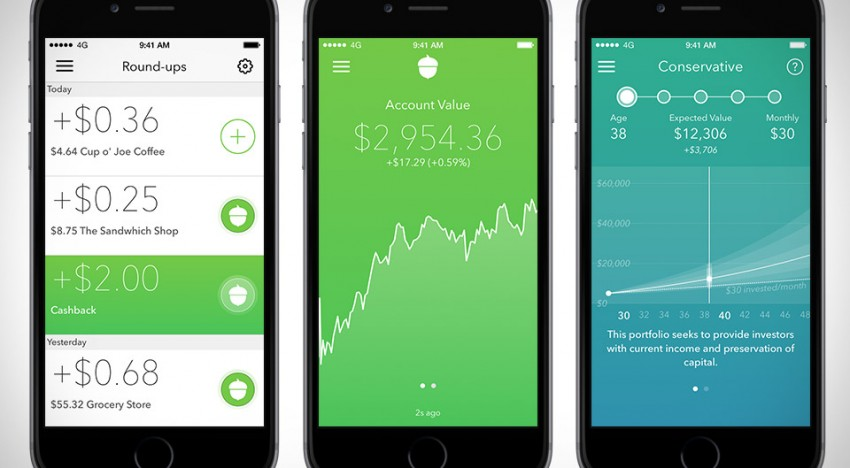
\includegraphics[height=.65\textheight]{assets/acorns.jpg}
            \caption{Acorns}
            \label{fig:acorns}
        \end{figure}
    \end{frame}

    \begin{frame}
        \frametitle{Prior Knowledge}

        \begin{itemize}
            \item I've had mediocre money management skills in the past.
            \item I would basically ballpark expenses and such.
            \item Although this would suffice in college, it would not last me in the real world long.
        \end{itemize}
    \end{frame}

    \begin{frame}
        \frametitle{Goals}

        \begin{itemize}
            \item To keep a reliable budget for the entirety of the semester.
            \item To be able to update my budget when I graduate easily.
        \end{itemize}
    \end{frame}

    \begin{frame}
        \frametitle{Resources}

        \begin{itemize}
            \item All of the learning (besides a couple of articles online) came from experimenting.
        \end{itemize}
    \end{frame}

    \begin{frame}
        \frametitle{Goal Accomplishment}

        \begin{itemize}
            \item I successfully created a budget within EmPower.

                \begin{itemize}
                    \item It handles all my weekly expenses (i.e., grocery shopping), monthly expenses (i.e., utilities or internet), and other miscellaneous expenses (entertainment).
                \end{itemize}

            \item I also was able to save a considerate amount into Acorns.

            \item The EmPower/Acorns system will be very useful when I graduate and move onto full time.
        \end{itemize}
    \end{frame}

    \begin{frame}
        \frametitle{Goal Not Accomplishment (Yet)}

        \begin{itemize}
            \item Sticking to my budget was very hard. Some months I would hit the price point, other times I would miss it by orders of magnitude.
            \item I would sometimes pull money out of my savings account a little prematurely.
        \end{itemize}
    \end{frame}


    \begin{frame}
        \frametitle{Lessons Learned}

        The lesson I learned that was most valuable to me was to check my budget everyday. If I don't check it daily, I won't know how much I can or cannot spend. This could be for better or worse.

    \end{frame}

    \begin{frame}
        \frametitle{In Closing}

        All question, comments, and insults can be directed towards me:

        \begin{center}
            \begin{description}
                \item[\faComment] \href{mailto:starikov@mst.edu}{starikov@mst.edu}
                \item[\faLinkedin] \href{https://www.linkedin.com/in/illyastarikov/}{Illya Starikov}
                \item[\faGithub] \href{https://github.com/IllyaStarikov/}{Illya Starikov}
                \item[\faRss] \href{https://freneticarray.com/}{FreneticArray.com}
            \end{description}
        \end{center}
    \end{frame}
\end{darkframes}
\end{document}
